\documentclass[border=20pt, tikz]{standalone}
\usepackage{amsmath}
\usetikzlibrary{calc, arrows.meta}

% =========================================================
% GLOBAL SETTINGS
% Applies uniformly to all diagrams on all pages
% (Note: No blank lines allowed inside \tikzset)
% =========================================================
\tikzset{
    glass/.style={fill=cyan!20, draw=cyan!70!blue, thick, fill opacity=0.35, line join=round},
    glassfront/.style={fill=cyan!30, draw=cyan!80!blue, thick, fill opacity=0.6, line join=round},
    axis/.style={thick, -{Latex[length=3mm, width=2mm]}},
    common settings/.style={
        font=\sffamily\small,
        x={(0.9cm, -0.15cm)}, 
        y={(0cm, 1cm)}, 
        z={(-0.6cm, -0.5cm)}
    }
}

\begin{document}


% =========================================================
% PAGE 3: NDC CUBE
% =========================================================
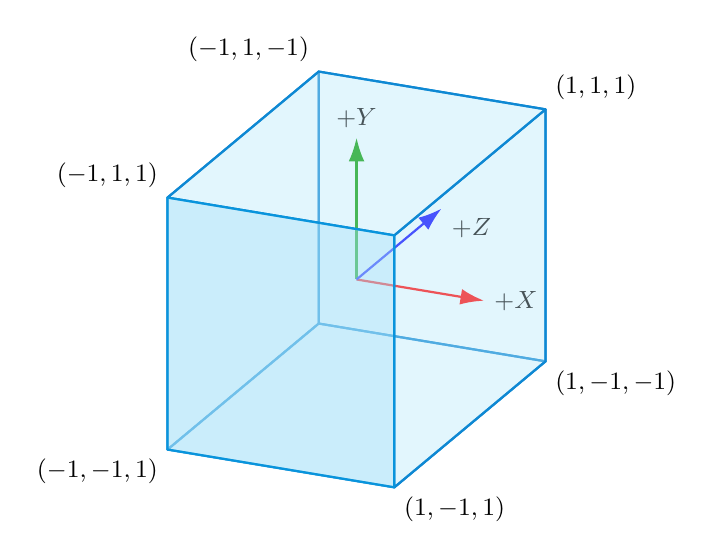
\begin{tikzpicture}[common settings]
    
    \def\c{1.6} % Cube scale for matching visual weight
    
    % Back Face (z=-1) & Hidden Side Faces
    \path[glass] (-\c,-\c,-\c) -- (\c,-\c,-\c) -- (\c,\c,-\c) -- (-\c,\c,-\c) -- cycle; % Back
    \path[glass] (-\c,-\c,-\c) -- (-\c,-\c,\c) -- (-\c,\c,\c) -- (-\c,\c,-\c) -- cycle; % Left
    \path[glass] (-\c,-\c,-\c) -- (\c,-\c,-\c) -- (\c,-\c,\c) -- (-\c,-\c,\c) -- cycle; % Bottom
    
    % Coordinate Axes inside the cube
    \draw[axis, red] (0,0,0) -- (1.8,0,0) node[right, text=black] {$+X$};
    \draw[axis, green!60!black] (0,0,0) -- (0,1.8,0) node[above, text=black] {$+Y$};
    \draw[axis, blue] (0,0,0) -- (0,0,-1.8) node[below right, text=black] {$+Z$};

    % Front Face (z=1) & Visible Side Faces
    \path[glass] (\c,-\c,-\c) -- (\c,-\c,\c) -- (\c,\c,\c) -- (\c,\c,-\c) -- cycle; % Right
    \path[glass] (-\c,\c,-\c) -- (\c,\c,-\c) -- (\c,\c,\c) -- (-\c,\c,\c) -- cycle; % Top
    \path[glassfront] (-\c,-\c,\c) -- (\c,-\c,\c) -- (\c,\c,\c) -- (-\c,\c,\c) -- cycle; % Front

    % Math Labels
    \node[above left] at (-\c, \c, -\c) {$(-1, 1, -1)$};  % Back top left
    \node[above right] at (\c, \c , -\c) {$(1, 1, 1)$};     % Front top right
    \node[above left] at (-\c, \c, \c) {$(-1, 1, 1)$};    % Front top left
    \node[below left] at (-\c, -\c, \c) {$(-1, -1, 1)$};  % Front bottom left
    \node[below right] at (\c, -\c, \c) {$(1, -1, 1)$};   % Front bottom right
    \node[below right] at (\c, -\c, -\c) {$(1, -1, -1)$}; % Back bottom right
    
\end{tikzpicture}

\end{document}